
\begin{figure}[H]
\begin{center}
\resizebox{0.5\textwidth}{!}
{
\begin{pspicture}(0,-2.0159376)(15.188437,2.0159376)
\psline[linewidth=0.04cm](0.1684375,-1.0303125)(15.168438,-1.0303125)
\psline[linewidth=0.04cm,arrowsize=0.05291667cm 2.0,arrowlength=1.4,arrowinset=0.4]{->}(3.1684375,0.9696875)(3.1684375,-1.0303125)
\psline[linewidth=0.04cm,arrowsize=0.05291667cm 2.0,arrowlength=1.4,arrowinset=0.4]{->}(6.1684375,-0.0303125)(6.1684375,-1.0303125)
\psline[linewidth=0.04cm,arrowsize=0.05291667cm 2.0,arrowlength=1.4,arrowinset=0.4]{->}(9.168438,-0.0303125)(9.168438,-1.0303125)
\psline[linewidth=0.04cm,arrowsize=0.05291667cm 2.0,arrowlength=1.4,arrowinset=0.4]{->}(12.168438,0.9696875)(12.168438,-1.0303125)
\psline[linewidth=0.04cm](6.1684375,-0.0303125)(7.4684377,-0.0303125)
\psline[linewidth=0.04cm](7.9684377,-0.0303125)(9.168438,-0.0303125)
\psline[linewidth=0.04cm](3.1684375,0.9696875)(8.168438,0.9696875)
\psline[linewidth=0.04cm](9.168438,0.9696875)(12.168438,0.9696875)
\pscircle[linewidth=0.04,dimen=outer](7.7184377,0.0196875){0.25}
\pscircle[linewidth=0.04,dimen=outer](8.668438,0.9696875){0.5}
\psline[linewidth=0.04cm,arrowsize=0.05291667cm 2.0,arrowlength=1.4,arrowinset=0.4]{->}(7.4684377,-0.2303125)(8.068438,0.3696875)
\psline[linewidth=0.04cm,arrowsize=0.05291667cm 2.0,arrowlength=1.4,arrowinset=0.4]{->}(8.168438,0.4696875)(9.268437,1.6696875)
\usefont{T1}{ptm}{m}{n}
\rput(7.9475,-0.4553125){\LARGE $\Delta U$}
\usefont{T1}{ptm}{m}{n}
\rput(7.974375,1.7446876){\LARGE Source $I$}
\usefont{T1}{ptm}{m}{n}
\rput(3.179375,-1.4553125){\LARGE A}
\usefont{T1}{ptm}{m}{n}
\rput(6.223906,-1.4553125){\LARGE M}
\usefont{T1}{ptm}{m}{n}
\rput(9.084687,-1.4553125){\LARGE N}
\usefont{T1}{ptm}{m}{n}
\rput(12.147187,-1.4553125){\LARGE B}
\usefont{T1}{ptm}{m}{n}
\rput(1.4175,-1.7553124){\LARGE $\rho$}
\usefont{T1}{ptm}{m}{n}
\rput(1.5075,-0.4553125){\LARGE $\rho=\infty$}
\end{pspicture} 
}

\caption{Four point measurement}
\label{fig:dc01}
\end{center}
\end{figure}
Resistivity $\rho$ of the subsurface derived from $I$ (which is known), $\Delta U$ (which is measured) and the geometrical factor $K$ (which is also known).

\subsubsection*{Frequently used electrode arrays}

\begin{figure}[H]
\begin{center}
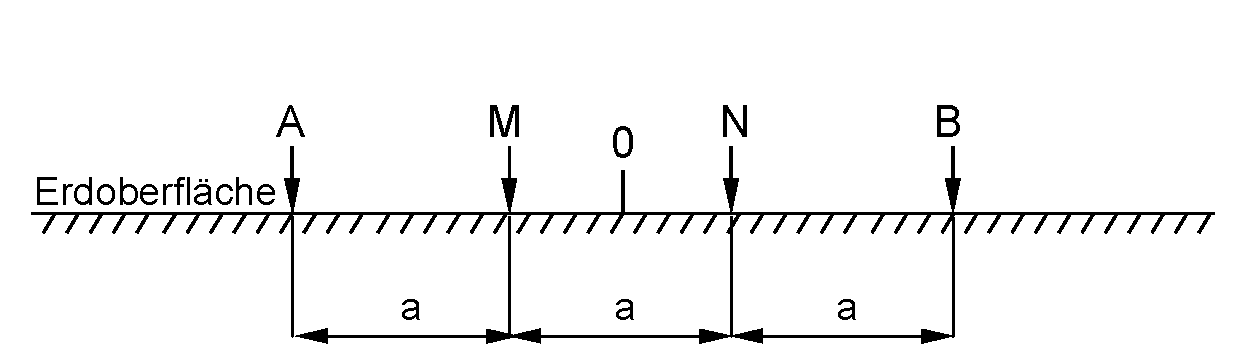
\includegraphics[width=0.5\textwidth]{Wenner.png}
a)
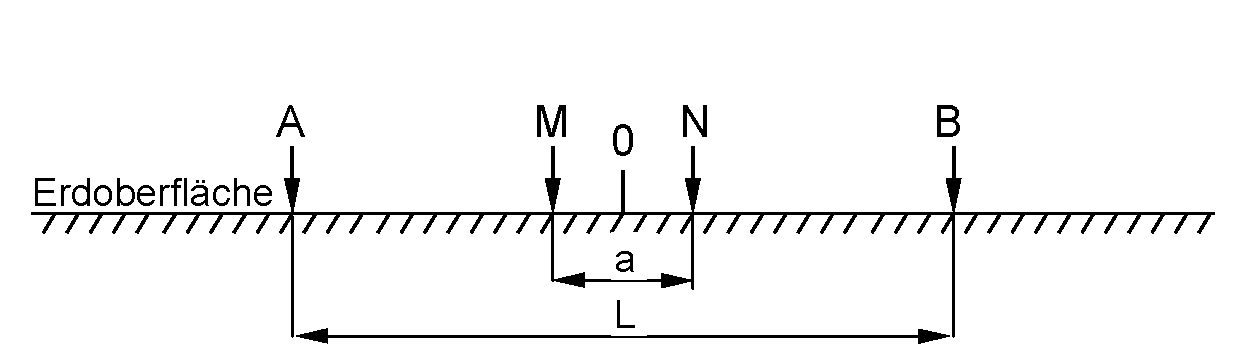
\includegraphics[width=0.5\textwidth]{Schlumberger.png}
b)
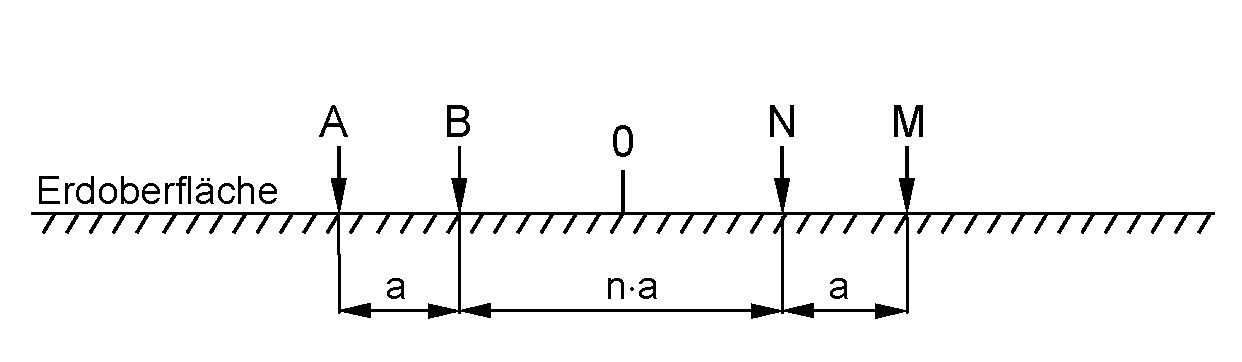
\includegraphics[width=0.5\textwidth]{Dipoldipol.png}
c)
\caption{a) Wenner, Half-Wenner; b) Schlumberger, Half-Schlumberger; c) Dipole-dipole, source???}
\label{fig:dc02}
\end{center}
\end{figure}

Industrial standard of measuring is via an \textit{Multielectrode array}.


\subsection{Basic equations of DC-resistivity}
The first assumption of DC-resistivity methods and the major difference to EM-methods is the assumption of stationary currents:
\begin{align*}
\frac{\partial}{\partial t}=0
\end{align*}
The fields do not depend on time.

Looking at the \textit{Maxwell's equations}:
\begin{align}
\nabla\times\vec{E}=\frac{\partial \vec{B}}{\partial t}=0
\end{align}
This means irrotational electric field and from that follows, that the electric field vector can be derived by a scalar potential:

\begin{equation}
\vec{E}=-\nabla V \label{eq:2-2}
\end{equation}
Insert equation \eqref{eq:2-2} into eq. \eqref{eq:1-2}:

\begin{equation}
\vec{j}=-\sigma \nabla V\label{eq:2-3}
\end{equation}
\textit{Continuity equation:}
\begin{equation}
\nabla\cdot\vec{j}+\frac{\partial q}{\partial t}=0
\end{equation}
Now new charges are generated in the course of time
\begin{equation}
\nabla\cdot\vec{j}=0 \label{eq:2-5}
\end{equation}
which is valid outside of the source.

If we insert eq. \eqref{eq:2-3} into \eqref{eq:2-5}:
\begin{align*}
-\nabla\cdot(\sigma\nabla V)&=0\\
\nabla\sigma\nabla V + \sigma\nabla^2V&=0
\end{align*}
$\nabla\sigma=0$ for areas with constant conductivity, so:
\begin{equation}
\nabla^2 V=0\label{eq:lapleq}
\end{equation}
which is called the \textit{Laplace-equation}, the basic equation of DC-resistivity.

Derivation of solutions of this elliptic partial differential equation using  different boundary conditions:

Assume a current source with strength $I$ at point $\vec{r}_0$, then the spatial current distribution can be given as:$\nabla\cdot\vec{j}=I\delta(\vec{r}-\vec{r}_0$
and so:
\begin{equation}
\nabla\cdot(\sigma\nabla V)=-I\delta(\vec{r}-\vec{r}_0)
\end{equation}
This equation can be solved numerically for arbitrary distribution of conductivity ratio.


\subsubsection{Potential of a current electrode}

\begin{figure}[H]
\begin{center}
\resizebox{0.5\textwidth}{!}
{
\begin{pspicture}(0,-3.02)(10.189688,1.02)
\psline[linewidth=0.04cm](0.0,0.0)(8.0,0.0)
\rput{-180.0}(8.0,0.0){\psarc[linewidth=0.04,linestyle=dashed,dash=0.16cm 0.16cm](4.0,0.0){3.0}{0.0}{180.0}}
\psline[linewidth=0.04cm,arrowsize=0.05291667cm 2.0,arrowlength=1.4,arrowinset=0.4]{->}(4.0,1.0)(4.0,0.0)
\psline[linewidth=0.04cm,arrowsize=0.05291667cm 2.0,arrowlength=1.4,arrowinset=0.4]{->}(4.0,0.0)(1.2,-1.0)
\psline[linewidth=0.04cm,arrowsize=0.05291667cm 2.0,arrowlength=1.4,arrowinset=0.4]{->}(4.0,0.0)(4.0,-3.0)
\psline[linewidth=0.04cm,arrowsize=0.05291667cm 2.0,arrowlength=1.4,arrowinset=0.4]{->}(4.0,0.0)(6.9,-1.0)
\psline[linewidth=0.04cm,arrowsize=0.05291667cm 2.0,arrowlength=1.4,arrowinset=0.4]{->}(4.0,0.0)(1.7,-1.9)
\psline[linewidth=0.04cm,arrowsize=0.05291667cm 2.0,arrowlength=1.4,arrowinset=0.4]{->}(4.0,0.0)(6.3,-1.9)
\psline[linewidth=0.04cm,arrowsize=0.05291667cm 2.0,arrowlength=1.4,arrowinset=0.4]{->}(4.0,0.0)(2.7,-2.7)
\psline[linewidth=0.04cm,arrowsize=0.05291667cm 2.0,arrowlength=1.4,arrowinset=0.4]{->}(4.0,0.0)(5.3,-2.7)
\usefont{T1}{ptm}{m}{n}
\rput(8.788125,-0.595){equipotential surface}
\usefont{T1}{ptm}{m}{n}
\rput(2.1721876,-0.195){current flow}
\psline[linewidth=0.04cm,arrowsize=0.05291667cm 2.0,arrowlength=1.4,arrowinset=0.4]{->}(7.2,-0.6)(7.0,-0.5)
\psline[linewidth=0.04cm,arrowsize=0.05291667cm 2.0,arrowlength=1.4,arrowinset=0.4]{->}(1.7,-0.4)(1.8,-0.7)
\rput{-180.0}(8.0,0.0){\psarc[linewidth=0.04,linestyle=dashed,dash=0.16cm 0.16cm](4.0,0.0){2.0}{0.0}{180.0}}
\end{pspicture} 
}
\caption{Single current source}
\label{fig:singlesource}
\end{center}
\end{figure}

Using \textit{Ohm's law}: $\vec{E}=\rho\vec{j}=\rho\frac{I}{2\pi r^2}$, where $2\pi r^2$ is the surface of the half sphere. Using $E=-\frac{dV}{dr}$ follows the potential of a homogeneous half space:
\begin{equation}
V=\frac{\rho I}{2\pi r}
\end{equation}

\begin{figure}[H]
\begin{center}
\resizebox{0.5\textwidth}{!}
{
\begin{pspicture}(0,-2.9690626)(13.175938,2.9890625)
\psline[linewidth=0.04cm](0.0,1.0509375)(8.0,1.0509375)
\psline[linewidth=0.04cm](2.0,-1.9490625)(4.0,2.0509374)
\psline[linewidth=0.04cm](4.0,2.0509374)(5.2,2.0509374)
\psline[linewidth=0.04cm](6.0,2.0509374)(6.8,2.0509374)
\psline[linewidth=0.04cm,linestyle=dashed,dash=0.16cm 0.16cm,arrowsize=0.05291667cm 2.0,arrowlength=1.4,arrowinset=0.4]{->}(6.8,2.0509374)(9.3,2.0509374)
\usefont{T1}{ptm}{m}{n}
\rput(10.955313,2.3959374){\Large $c_2\rightarrow\infty$}
\psdots[dotsize=0.16](2.0,-1.9490625)
\psline[linewidth=0.04cm,arrowsize=0.05291667cm 2.0,arrowlength=1.4,arrowinset=0.4]{->}(2.0,-1.9490625)(3.0,-1.9490625)
\psline[linewidth=0.04cm,arrowsize=0.05291667cm 2.0,arrowlength=1.4,arrowinset=0.4]{->}(2.0,-1.9490625)(2.0,-0.9490625)
\psline[linewidth=0.04cm,arrowsize=0.05291667cm 2.0,arrowlength=1.4,arrowinset=0.4]{->}(2.0,-1.9490625)(1.0,-1.9490625)
\psline[linewidth=0.04cm,arrowsize=0.05291667cm 2.0,arrowlength=1.4,arrowinset=0.4]{->}(2.0,-1.9490625)(2.0,-2.9490626)
\pscircle[linewidth=0.04,linestyle=dashed,dash=0.16cm 0.16cm,dimen=outer](2.0,-1.9490625){1.0}
\psline[linewidth=0.04cm,arrowsize=0.05291667cm 2.0,arrowlength=1.4,arrowinset=0.4]{->}(2.0,-1.9490625)(2.7,-2.6490624)
\psline[linewidth=0.04cm,arrowsize=0.05291667cm 2.0,arrowlength=1.4,arrowinset=0.4]{->}(2.0,-1.9490625)(1.3,-2.6490624)
\psline[linewidth=0.04cm,arrowsize=0.05291667cm 2.0,arrowlength=1.4,arrowinset=0.4]{->}(2.0,-1.9490625)(1.3,-1.2490625)
\psline[linewidth=0.04cm,arrowsize=0.05291667cm 2.0,arrowlength=1.4,arrowinset=0.4]{->}(2.0,-1.9490625)(2.7,-1.3490624)
\usefont{T1}{ptm}{m}{n}
\rput(3.5653124,-1.7040625){\Large $c_1$}
\pscircle[linewidth=0.04,dimen=outer](5.6,2.0509374){0.4}
\psline[linewidth=0.04cm,arrowsize=0.05291667cm 2.0,arrowlength=1.4,arrowinset=0.4]{->}(5.3,1.6509376)(6.0,2.5509374)
\usefont{T1}{ptm}{m}{n}
\rput(5.6876564,2.7809374){\large Source}
\end{pspicture} 
}

\caption{Mise-\`a-la-Masse method}
\label{fig:misemasse}
\end{center}
\end{figure}

In the case of the \textit{Mise-\`a-la-Masse method} the potential of the homogeneous full space is:
\begin{equation}
V=\frac{\rho I}{4\pi r}
\end{equation}

The same result can be derived by using the Laplace-equation \eqref{eq:lapleq} and the use of spherical coordinates:
\begin{align*}
\nabla^2 V=\frac{d^2V}{dr^2}+\frac{2}{r}\frac{dV}{dr}
\end{align*}
From the symmetry of the system the potential is a function of the distance to the source $r$ only. Multiplying by $r^2$ and integrating, we get:
\begin{align*}
\frac{dV}{dr}=\frac{c_1}{r^2}
\end{align*}
Integrating over $r$ again leads to the solution:
\begin{align*}
V=-\frac{c_1}{r}+c_2 && c_1,c_2 = const.
\end{align*}
To determine the constants we have to use boundary conditions: From $\lim_{r \to \infty} V(r) = 0$ follows that $c_2=0$. Using the current density: $j=\frac{I}{A}\Leftrightarrow I=jA$:
\begin{equation*}
I=4\pi r^2j=-4\pi r^2\sigma\frac{dV}{dr}=-4\pi\sigma c_1
\end{equation*}
From this equation we can derive $c_1$:
\begin{equation}
V=\frac{I\rho}{4\pi r}
\end{equation}

\subsection*{Boundary equations}
Boundary with different conductivities.

\begin{figure}[H]
\begin{center}
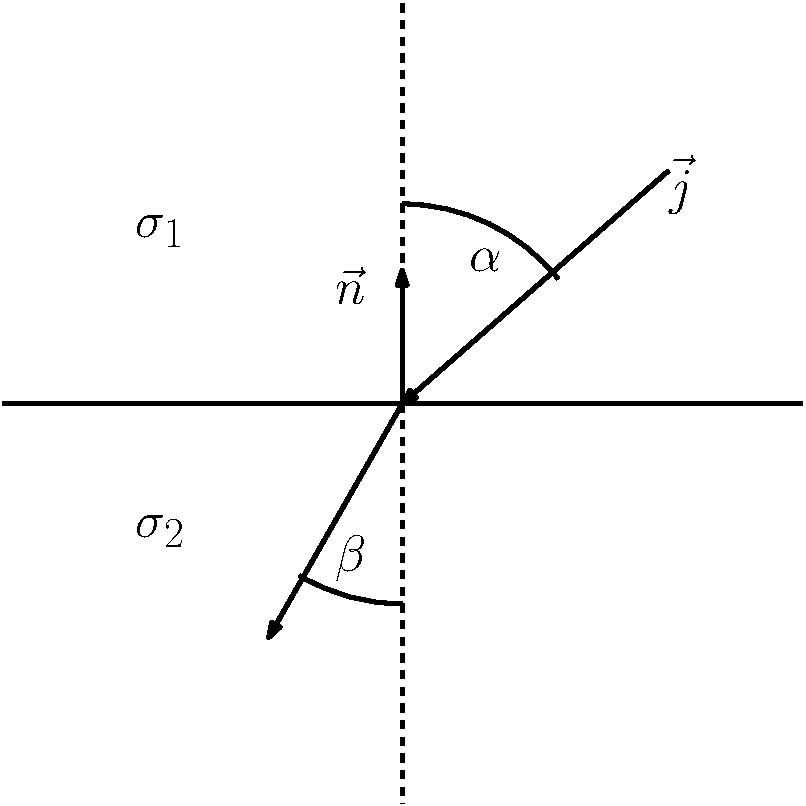
\includegraphics[scale=0.5]{figs/grenz.pdf}
\caption{Boundary with dip angles GEOING s5}
\label{fig:bound01}
\end{center}
\end{figure}

Two boundary conditions which must hold at any contact between two regions of different conductivity.
\begin{itemize}
\item Potential is continuous across the boundary
\item $j_n$ is also continuous.
\end{itemize}
\begin{align*}
V^1=V^2, ~~~\left(\frac{\partial V}{\partial x}\right)^1=\left(\frac{\partial V}{\partial x}\right)^2,~~~ j_n^1=j_n^2
\end{align*}
\begin{align*}
E_t^1=E_t^2, ~~~\sigma_1 E_n^1=\sigma_2 E_n^2
\end{align*}
\begin{align*}
\sigma_1 \frac{E_n^1}{E_t^1}&=\sigma_2 \frac{E_n^2}{E_t^2}\\
\sigma_1\cot\alpha&=\sigma_2\cot\beta\\
\frac{\tan\alpha}{\tan\beta}&=\frac{\sigma_1}{\sigma_2}
\end{align*}
Current line is bent towards to the normal if the resistivity of the second medium $\rho_2$ is larger than the one of the first medium $\rho_1$.

\begin{figure}[H]
\begin{minipage}{0.45\textwidth}
	\centering
	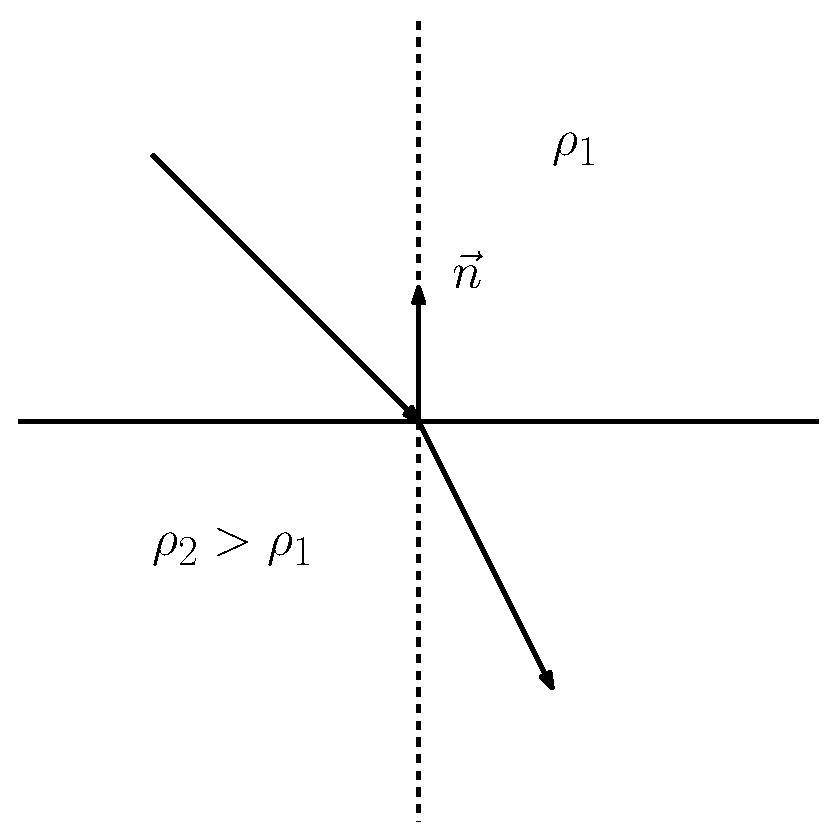
\includegraphics[width=\textwidth]{grenz_02.eps}
\end{minipage}
\hspace{0.05\textwidth}
\begin{minipage}{0.45\textwidth}
\centering
	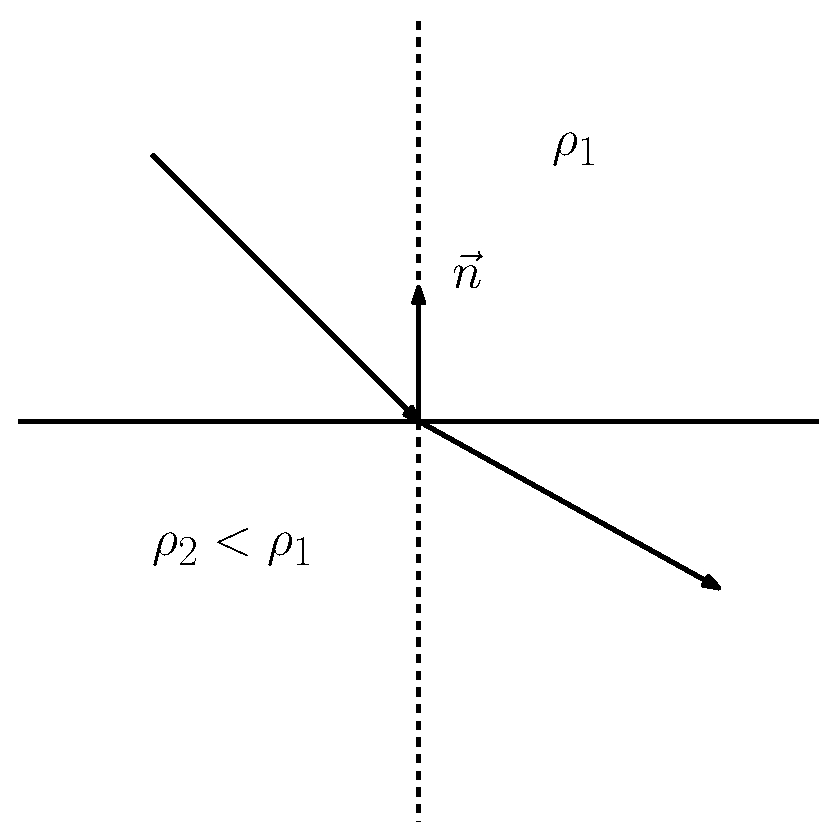
\includegraphics[width=\textwidth]{grenz_03.eps}
\end{minipage}
\begin{minipage}[t]{0.45\textwidth}
\centering
	\captionof{figure}{Bending towards normal}
	\label{bound_01}
\end{minipage}
\hspace{0.05\textwidth}
\begin{minipage}[t]{0.45\textwidth}
	\centering
	\captionof{figure}{Bending away from normal}
	\label{bound_02}
\end{minipage}
\end{figure}

\subsubsection{Potential distribution at the surface of a horizontally stratified earth (Solution of the Laplace equation \eqref{eq:lapleq})}
\label{ch:2.1.2}
Starting with a \textit{model}:

\begin{figure}[H]
\begin{center}
\resizebox{0.3\textwidth}{!}
{
\begin{pspicture}(0,-3.0375)(6.541875,3.0175)
\psline[linewidth=0.04cm](0.0,1.6975)(4.0,1.6975)
\psline[linewidth=0.04cm](0.0,0.6975)(4.0,0.6975)
\psline[linewidth=0.04cm](0.0,-0.3025)(4.0,-0.3025)
\psline[linewidth=0.04cm](0.0,-2.3025)(4.0,-2.3025)
\usefont{T1}{ptm}{m}{n}
\rput(0.95734376,1.2275){\large $\rho_1$}
\usefont{T1}{ptm}{m}{n}
\rput(0.95734376,0.2275){\large $\rho_2$}
\usefont{T1}{ptm}{m}{n}
\rput(0.94734377,-2.7725){\large $\rho_n$}
\usefont{T1}{ptm}{m}{n}
\rput(3.4173439,-2.7725){\large $h_n\rightarrow\infty$}
\usefont{T1}{ptm}{m}{n}
\rput(3.0173438,0.2275){\large $h_2$}
\usefont{T1}{ptm}{m}{n}
\rput(3.0173438,1.2275){\large $h_1$}
\psline[linewidth=0.04cm,arrowsize=0.05291667cm 2.0,arrowlength=1.4,arrowinset=0.4]{->}(2.0,2.6975)(2.0,1.6975)
\psline[linewidth=0.04cm](2.0,2.6975)(3.2,2.6975)
\psline[linewidth=0.04cm](3.2,2.8975)(3.2,2.4975)
\psline[linewidth=0.04cm](3.4,2.9975)(3.4,2.3975)
\psline[linewidth=0.04cm](3.4,2.6975)(4.0,2.6975)
\psline[linewidth=0.04cm,linestyle=dashed,dash=0.16cm 0.16cm,arrowsize=0.05291667cm 2.0,arrowlength=1.4,arrowinset=0.4]{->}(4.0,2.6975)(5.5,2.6975)
\usefont{T1}{ptm}{m}{n}
\rput(5.9414062,2.7025){$\infty$}
\psdots[dotsize=0.1](1.0,-0.8025)
\psdots[dotsize=0.1](1.0,-1.1025)
\psdots[dotsize=0.1](1.0,-1.4025)
\psdots[dotsize=0.1](3.0,-0.8025)
\psdots[dotsize=0.1](3.0,-1.1025)
\psdots[dotsize=0.1](3.0,-1.4025)
\end{pspicture} 
}

\caption{Model of $n$ layer structure}
\label{fig:model01}
\end{center}
\end{figure}

The subsurface consists of finite number of layers with the last layer having infinite layer thickness ( $h_n\rightarrow\infty$ ). We assume that $\rho_i$ is isotropic (no dependence of the direction of measurement). The field is generated by a point source with the current $I$ is a direct current.

Starting from the Laplace equation with potential $V$:
\begin{equation}
\frac{\partial^2 V}{\partial x^2}+\frac{\partial^2 V}{\partial y^2}+\frac{\partial^2 V}{\partial z^2}=0
\end{equation}
In cylindrical coordinates ($r,\theta,z$):
\begin{equation}
\frac{\partial^2 V}{\partial r^2}+\frac{1}{r}\frac{\partial V}{\partial r}+\frac{\partial^ V}{\partial z^2}+\frac{1}{r^2}\frac{\partial^2 V}{\partial\theta^2}=0
\end{equation}

The solution is symmetrical to the vertical axis, so $\frac{\partial V}{\partial \theta}=\frac{\partial^2 V}{\partial\theta^2}=0$, so $V(r,\theta,z)=V(r,z)$. So the Laplace equation to be solved reduces to:
\begin{equation}
\frac{\partial^2 V}{\partial r^2}+\frac{1}{r}\frac{\partial V}{\partial r}+\frac{\partial^ V}{\partial z^2}=0
\label{eq:laplcyl}
\end{equation}

Solution of \eqref{eq:laplcyl}. Ansatz:

\begin{equation}
V(r,z)=U(r)W(z) \label{eq:ansatz01}
\end{equation}
So the solution is the product of a function of $r$ alone and a function of $z$ alone. We substitute \eqref{eq:ansatz01} into \eqref{eq:laplcyl} and multiply all terms with $1/UW$:
\begin{align}
\underbrace{\frac{1}{UW}\frac{d^2 U}{dr^2}+\frac{1}{UW}\frac{DU}{dr}}_{\textrm{depends on } r}+\underbrace{\frac{1}{W}\frac{d^2 W}{dz^2}}_{\textrm{depends on } z}=0
\end{align}

This equation is satisfied, if
\begin{align}
\label{eq:ansatz03}
\frac{1}{U}\frac{d^2 U}{dr^2}+\frac{1}{Ur}\frac{DU}{dr}&=-\lambda^2\\ 
\frac{1}{W}\frac{d^2W}{dz^2}&=\lambda^2\label{eq:ansatz02}
\end{align}
where $\lambda$ is a real constant.

\subsubsection*{Solution of \eqref{eq:ansatz02}}

Using the Ansatz:
\begin{equation}
W=Ce^{-\lambda z}~~~,~~~ W=Ce^{\lambda z} \label{eq:ansatz05}
\end{equation}
where $C$ and $\lambda$ are arbitrary constants.
\subsubsection*{Solution of \eqref{eq:ansatz03}}

Using the Ansatz:
\begin{equation}
U=C J_0(\lambda r) \label{eq:ansatz06}
\end{equation}
with $J_0(\lambda r)$ the \textit{Bessel-function} of order zero.

\begin{figure}[H]
\begin{center}
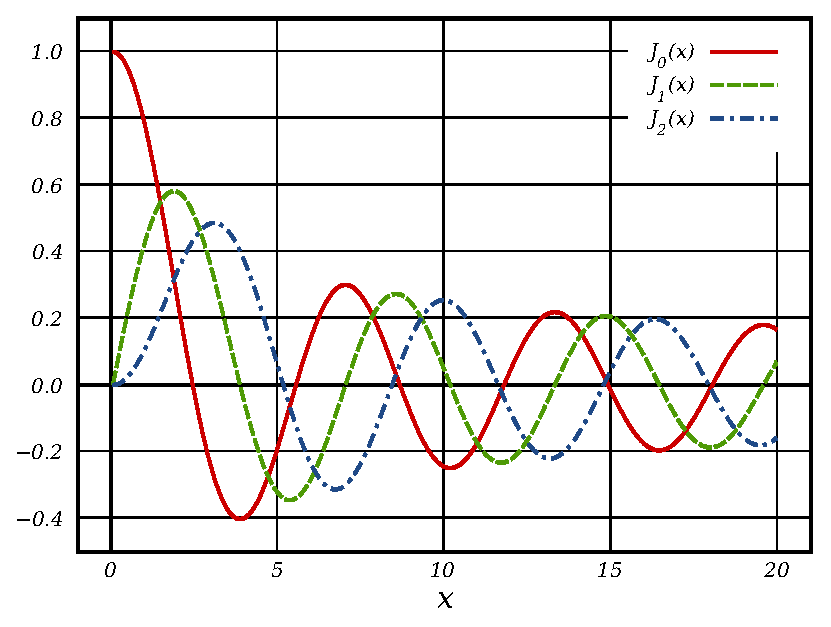
\includegraphics[width=0.5\textwidth]{besselfunctions.eps}
\caption{Bessel-functions source: $ https://de.wikipedia.org/wiki/Besselsche_Differentialgleichung$}
\label{fig:besself}
\end{center}
\end{figure}

We combine the two solutions (\eqref{eq:ansatz05} and \eqref{eq:ansatz06}) for the solution of \eqref{eq:laplcyl}:

\begin{equation}
V=Ce^{-\lambda z}J_0(\lambda r) ~~~,~~~ V=Ce^{\lambda z}J_0(\lambda r) \label{eq:ansatz07}
\end{equation}
$\lambda$ varies from $0$ to $\infty$ and $C$ varies in dependence of $\lambda$. Than we write a general solution of the potential \eqref{eq:laplcyl}:
\begin{equation}
V=\int\limits_{0}^{\infty}\left(\phi(\lambda)e^{-\lambda z}+\psi(\lambda)e^{\lambda z}\right)J_0(\lambda r) d\lambda \label{eq:sol-lapleq}
\end{equation}

Where $\phi(\lambda)$ and $\psi(\lambda)$ are arbitrary functions of $\lambda$.

\subsubsection*{Potential of homogeneous halfspace}
Starting of with the potential in cylindrical coordinates:
\begin{equation}
V=\frac{I\rho}{2\pi\sqrt{r^2+z^2}}\label{eq:2-20}
\end{equation}
Looking at the \textit{Lipschitz-Integral}:
\begin{equation}
\int\limits_{0}^{\infty}e^{-\lambda z}J_0(\lambda r)d\lambda=\frac{1}{\sqrt{r^2+z^2}} \label{eq:lipschitzint}
\end{equation}

Now using \eqref{eq:lipschitzint} we write \eqref{eq:2-20} as:
\begin{equation}
V=\frac{\rho_1 I}{2\pi}\int\limits_{0}^{\infty}e^{-\lambda z}J_0(\lambda r)d\lambda
\end{equation}

The general solution \eqref{eq:sol-lapleq} can now be written:
\begin{equation}
V=\frac{\rho_1 I}{2\pi}\int\limits_{0}^{\infty}\left(e^{-\lambda z}+\theta(\lambda)e^{-\lambda z}+X(\lambda)e^{\lambda z}\right) J_0(\lambda r)d\lambda \label{eq:sol-lapleq-2}
\end{equation}

Where $\theta(\lambda)$ and $X(\lambda)$ are arbitrary functions of $\lambda$, and $\phi(\lambda)=\frac{\rho_1 I}{2\pi}\left(1+\theta(\lambda)\right)$ and $\psi(\lambda)=\frac{\rho_1 I}{2\pi}X(\lambda)$.

The solutions of the form \eqref{eq:sol-lapleq-2} are valid in all layers but $\theta(\lambda)$ and $X(\lambda)$ can be different for each layer $i$:
\begin{equation}
V_i=\frac{\rho_1 I}{2\pi}\int\limits_{0}^{\infty}\left(e^{-\lambda z}+\theta_i(\lambda)e^{-\lambda z}+X_i(\lambda)e^{\lambda z}\right)J_0(\lambda r) d\lambda\label{eq:sol-lapleq-3}
\end{equation}

\subsubsection*{Adaption of the solution to the boundary conditions}

Assuming we are at the layer boundaries of $z=h_i$.


\begin{compactenum}[A)]
\item Potential \eqref{eq:sol-lapleq-3} is continious at each boundary plane in the subsurface:
\begin{equation}
V_i(r,h_i)=V_{i+1}(r,h_i)
\end{equation}
This equation can only be satisfied if the integrands on both sides are equal:
\begin{equation}
\theta_i(\lambda)e^{-\lambda h_i}+X_i(\lambda)e^{\lambda h_i}=\theta_{i+1}(\lambda)e^{-\lambda h_i}+X_{i+1}(\lambda)e^{\lambda h_i} \label{eq:boundary-2-23A}
\end{equation}
\item At each boundary plane $j_z$ the boundary condition must be fulfilled that:
\begin{equation}
j_z=-\frac{1}{\rho}\frac{\partial V}{\partial z}
\end{equation} 
and so
\begin{equation}
\frac{1}{\rho_i}\left(\left(1+\theta_i(\lambda)\right)e^{\lambda h_i}-X_i(\lambda)e^{\lambda h_i}\right)=\frac{1}{\rho_{i+1}}\left(\left(1+\theta_{i+1}(\lambda)\right)e^{\lambda h_i}-X_{i+1}(\lambda)e^{\lambda h_i}\right) \label{eq:boundary-2-23B}
\end{equation}
To satisfy this condition we differentiate the expression for the potential in the first layer \eqref{eq:2-20} with respect to $z$ and then substitute $z=0$:
\begin{equation}
\frac{1}{\rho_1}\frac{\partial V_1(r,0)}{\partial z}=0 ~~~,~ \textrm{for~~} r\neq 0
\end{equation}
We thus obtain the equation:
\begin{equation}
\int\limits_{0}^{\infty}\left(-1-\theta_1(\lambda)+X_1(\lambda)\right) J_0(\lambda_r)d\lambda=0
\end{equation}
\begin{equation}
\Rightarrow \theta_1(\lambda)=X_1(\lambda) \label{eq:boundary-2-23C}
\end{equation}

\item Near the current source the potential must approach to infinity
\begin{align*}
V_\infty=\frac{\rho I}{2\pi}\frac{1}{\sqrt{r^2+z^2}}
\end{align*}
which is approaching asymtotically to the potential for a layer extending to infinite height.

\item $V\rightarrow 0$ if $z\rightarrow\infty$ 
\begin{equation}
\Rightarrow X_n=0 \label{eq:boundary-2-23D}
\end{equation}
, because otherwise $e^{\lambda z}$ would drive the potential to an infinite value at an infinite depth.

\end{compactenum}

The set of equations \eqref{eq:boundary-2-23A} - \eqref{eq:boundary-2-23D} provides a system of $2n$ equation in $2n$ unknown functions $\theta(\lambda)$ and $X(\lambda)$. To obtain the solution subsitute \eqref{eq:boundary-2-23C} into \eqref{eq:boundary-2-23A} and \eqref{eq:boundary-2-23B} and subsitute \eqref{eq:boundary-2-23D} into \eqref{eq:boundary-2-23A} and \eqref{eq:boundary-2-23B}.

For brevity, we introduce the notations:
\begin{align*}
u_i=e^{\lambda h_i}, v_i=\frac{1}{u_i}, p_i=\frac{\rho_i}{\rho_{i+1}}
\end{align*}
The system of equations then become:
\begin{align*}
(u_1+v_1)\theta_1-u_2\theta_2-v_2X_2&=0\\
(v_1-u_1)\theta_1+p_1u_1\theta_2-p_1v_1X_2&=(1-p_1)u_1\\
\vdots~~~~~~~~~~~~~~~~~~~~&\vdots\\
u_{n-1}\theta_{n-1}+v_{n-1}X_{n-1}-u_{n-1}\theta_n&=0\\
-u_{n-1}\theta_{n-1}+v_{n-1}X_{n-1}+p_{n-1}u_{n-1}\theta_n-p_{n-1}v_{n-1}X_n&=(1-p_{n-1})u_{n-1}
\end{align*}
Solution of the equations by applying \textit{Cramer's rule}. For example: Solution of a two layer case (layer 1: $\rho_1, h_1$, layer 2: $\rho_2$):
\begin{align*}
\theta_1&=\frac{ku}{1-ku} && \theta_2=\frac{k(1+u)}{1-ku}\\
X_1&=\theta_1 && X_2=0
\end{align*}
with $u=e^{-2\lambda h_1}$ and the \textit{reflection coefficient of DC} $k=\frac{\rho_2-\rho_1}{\rho_2+\rho_1}$

Interesting is the potential at the surface of the earth, with $z=0$ and \eqref{eq:boundary-2-23C}:
\begin{align}
V_0=V_1(r,z)&=\frac{\rho_1 I}{2\pi}\int\limits_{0}^{\infty}\left(1+2\theta_1\right)J_0(\lambda r)d\lambda\\
&=\frac{\rho_1 I}{2\pi}\int\limits_{0}^{\infty}K(\lambda)J_0(\lambda r)d\lambda
\end{align}
where $K(\lambda)$ is the \textit{Slichter-function}.

We consider the Lipschitz-integral:
\begin{equation}
\int\limits_{0}^{\infty}e^{-\lambda z}J_0(\lambda r)d\lambda=\frac{1}{\sqrt{r^2+z^2}}\stackrel{i=0}= \int\limits_{0}^{\infty}J_0(\lambda r)d\lambda=\frac{1}{r}
\end{equation}
\eqref{eq:sol-lapleq-3} can now be written in the form:
\begin{equation}
V_0(r)=\underbrace{\frac{I}{2\pi}\left(\frac{\rho_1}{r}\right.}_{\textrm{first layer}}\left.+\int\limits_{0}^{\infty}(T(\lambda)-\rho_1)J_0(\lambda r)d\lambda\right)
\end{equation}
with $T(\lambda)=\rho_1(1+2\theta_1(\lambda))$
Example/reminder for four point measurement:
\begin{align*}
V_1=\frac{I\rho}{2\pi}\left(\frac{1}{AM}-\frac{1}{BM}\right)
\label{eq:V0}
\end{align*}

\subsubsection{Derivation of a formula for the apparent resistivity}
Take an arbitrary DC-Array (compare Fig. \ref{fig:dc01}). Then
\begin{align*}
\Delta U=\frac{I\rho}{2\pi}\left(\frac{1}{AM}-\frac{1}{AN}-\frac{1}{BM}+\frac{1}{BN}\right)
\end{align*}
\begin{align*}
\rho_a=k\frac{\Delta U}{I}
\end{align*}
where $k$ is the geometrical factor.
If we look at experimental data with an error of 1\% for the distances between the electrodes, the error in $\rho_a$ would be 2\%. But 10\% error in the lateral direction of the electrodes results only in 1\% error in $\rho_a$.

In case of the Schlumberger array ($L=AM+MN/2$ and $a=MN$, $a\ll L$) we get a voltage decrease in U:
\begin{align*}
U&=2\left(V_0(\frac{L}{2}-\frac{a}{2}\right)-V_0\left(\frac{L}{2}+\frac{a}{2}\right)\\
&\approx -2a\frac{\partial V_0}{\partial r}\bigg|_{r=L/2}
\end{align*}
and the geometrical factor in case of Schlumberger $k=\frac{\pi}{a}\left(\left(\frac{L}{2}\right)^2-\left(\frac{a}{2}\right)^2\right)$
\begin{align*}
\rho_a(L/2)=K\frac{U}{I}=\frac{2\pi}{I}\left(\frac{L}{2}\right)^2\frac{\partial V_0}{\partial r}
\end{align*}
with $\frac{d}{dx}J_0(x)=-J_1(x)$. From eq. 2.25!!!!:

\begin{equation}
\rho_a(L/2)=\rho_1+\left(\frac{L}{2}\right)^2\underbrace{\int\limits_{0}^{\infty}(T(\lambda)-\rho_1)J_1(\lambda L/2)\lambda d\lambda}_{\textrm{Stefanescu-Integral}} \label{eq:rho_a_01}
\end{equation}

The calculations of the model response $\rho_a(L/2)$ from given model parameters $(\rho_i,h_i)$ is a forward problem. 

Given:
\begin{figure}[H]
\begin{center}
\caption{Given parameters}
\label{fig:forwardgiven}
\end{center}
\end{figure}

Now two steps are neccessary:
\begin{itemize}
\item Calculation of $T(\lambda)$
\item Integration of \eqref{eq:rho_a_01} $\rightarrow$ Stefanescu-Integral
\end{itemize}

\subsubsection{Calculation of the resistivity transform $T(\lambda)$}

For a method for the determination of $T(\lambda)$ see chapter \ref{ch:2.1.2}. Then we calculate the solution of the equation system $\theta_i$ and $X_i$ and determine $T(\lambda)$ using $T(\lambda)=\rho_1(1+2\theta_1(\lambda))$. This procedure is too time consuming for a high number of layers.

Now we derive a recursion formula using the boundary conditions A to D from \ref{ch:2.1.2}. At first a new definition:

\begin{equation}
T_i(\lambda)=\rho_1\frac{1+\theta_1(\lambda)+X_i(\lambda)e^{2\lambda t_i-1}}{1+\theta_1(\lambda)-X_i(\lambda)e^{2\lambda t_i-1}}
\label{eq:Tlambda}
\end{equation}
with $i=1,2,\ddots,n$, $t_i=h_1+h_2+\ddots+h_i$ and $t_0=0$.

Because of \eqref{eq:boundary-2-23C}: $\theta_1(\lambda)=X_1(\lambda)$, we get: $T_1(\lambda)=T(\lambda)$.

Because of \eqref{eq:boundary-2-23D}: $X_n=0$, we get: $T_n(\lambda)=\rho_n$.\\

From the boundary conditions \eqref{eq:boundary-2-23A} and \eqref{eq:boundary-2-23B}:\\

\begin{compactenum}[a)]
\item $\theta_i(\lambda)e^{-\lambda t_i}+X_i(\lambda)e^{\lambda t_i}=\theta_{i+1}(\lambda)e^{-\lambda t_i}+X_{i+1}(\lambda)e^{\lambda t_i}$\\


\item $\frac{1}{\rho_i}\left(\left(1+\theta_i(\lambda)\right)e^{-\lambda t_i}-X_i(\lambda)\right)=\frac{1}{\rho_i}\left(\left(1+\theta_{i+1}(\lambda)\right)e^{-\lambda t_i}-X_{i+1}(\lambda)\right)$
\end{compactenum}

The next steps are:
\begin{itemize}
\item Add $e^{-\lambda t_i}$ on both sides of \eqref{eq:boundary-2-23A}
\item Divide each side over the corresponding side of \eqref{eq:boundary-2-23B}
\item Cancel the left part of the new equation by $X_i(\lambda)$
\end{itemize}
Then:

\begin{equation*}
\rho_i\frac{K_i(\lambda)+e^{2\lambda t_i}}{K_i(\lambda)-e^{2\lambda t_i}}=T_{i+1}(\lambda)
\end{equation*}
with $K_i(\lambda)=\frac{1+\theta_i(\lambda)}{X_i(\lambda)}$

Now the next step is to Solve the eq. \eqref{eq:Tlambda}, insert it and short translation and solving it for $T(\lambda)$:

\begin{equation}
T_i(\lambda)=\frac{T_{i+1}+\rho_i\tanh(\lambda h_i)}{1+\frac{T_{i+1}(\lambda)}{\rho_i}\tanh(\lambda h_i)}
\label{eq:Tlambda2}
\end{equation}
which is the \textit{recursion formula of PEKERIS}.

Now start with $T_n=\rho_n$, calculate step by step $T_i(\lambda)$ until $T_1(\lambda)=T(\lambda)$ $\rightarrow$ \textit{resistivity transform}

Illustration of eq. \eqref{eq:Tlambda2}:
\begin{align*}
\lambda=\frac{1}{L/2} && T_n(\lambda)=\rho_n
\end{align*}

Two extreme values:
\begin{align*}
L/2 \rightarrow 0 && L/2 \rightarrow \infty
\end{align*}

\subsubsection*{Two layer model}

\begin{figure}[H]
\begin{center}
\resizebox{0.4\textwidth}{!}
{
\begin{pspicture}(0,-0.87890625)(4.5009375,0.85890627)
\psline[linewidth=0.04cm](0.4809375,0.8389062)(4.4809375,0.8389062)
\psline[linewidth=0.04cm](0.4809375,-0.16109376)(4.4809375,-0.16109376)
\usefont{T1}{ptm}{m}{n}
\rput(1.6523438,0.34390625){$\rho_1=5\Omega m$}
\usefont{T1}{ptm}{m}{n}
\rput(1.6423438,-0.6560938){$\rho_2=10\Omega m$}
\usefont{T1}{ptm}{m}{n}
\rput(3.4423437,0.34390625){$\h_1=1 m$}
\end{pspicture} 
}

\caption{Two layer model}
\label{fig:2layermodel}
\end{center}
\end{figure}

$T_n(\lambda)=T_2(\lambda)=10\Omega m$

\begin{enumerate}
\item $L/2 \rightarrow 0$ $\Rightarrow \lambda \rightarrow \infty \Rightarrow \tanh(\infty)\rightarrow 1$
\begin{align*}
T(\lambda)=T_1(\lambda)=\frac{T_{2}+\rho_1\tanh(\lambda h_1)}{1+\frac{T_{2}(\lambda)}{\rho_1}\tanh(\lambda h_1)}=\frac{10+5}{1+10/5}=5\Omega m
\end{align*}
\item $L/2\rightarrow \infty \Rightarrow \lambda	\rightarrow 0 \Rightarrow \tanh(0)\rightarrow 0$
\begin{align*}
T_1(\lambda)=\frac{10+0}{1+0}=10\Omega m
\end{align*}
\end{enumerate}

\begin{figure}[H]
\begin{center}
\resizebox{0.5\textwidth}{!}
{
\begin{pspicture}(0,-2.4576561)(12.062813,2.4576561)
\psline[linewidth=0.04cm,arrowsize=0.05291667cm 2.0,arrowlength=1.4,arrowinset=0.4]{->}(1.7809376,-1.8407812)(9.780937,-1.8407812)
\psline[linewidth=0.04cm,arrowsize=0.05291667cm 2.0,arrowlength=1.4,arrowinset=0.4]{->}(1.7809376,-1.8407812)(1.7809376,2.2592187)
\psbezier[linewidth=0.04,linestyle=dashed,dash=0.16cm 0.16cm](1.7809376,1.1592188)(6.7809377,1.1592188)(4.6809373,-0.74078125)(8.780937,-0.74078125)
\usefont{T1}{ptm}{m}{n}
\rput(0.9323437,2.2642188){$T(1/(L/2))$}
\usefont{T1}{ptm}{m}{n}
\rput(10.542344,-2.2357812){$\lambda=(1/(L/2))$}
\usefont{T1}{ptm}{m}{n}
\rput(1.4334375,1.2642188){10}
\usefont{T1}{ptm}{m}{n}
\rput(1.3504688,-0.6357812){5}
\end{pspicture} 
}
\caption{??????}
\label{fig:lambdaTlambda}
\end{center}
\end{figure}

\subsubsection{Solution of the Stefanescu-Integral}
An analytical solution is not possible! One of the possibilities uses the linear filter method.
\paragraph{Basic Equations of the linear filter method: The fast HANKEL-transformation}

The calculation of a function $g(r)$ from $\rho(\lambda)$ by
\begin{equation}
g(r)=\int\limits_{0}^{\infty}\rho(\lambda)J_\nu(\lambda r)\lambda d\lambda
\label{eq:hankeltransform}
\end{equation}
is defined as the \textit{HANKEL-transformation}. It expresses any given function as the weighted sum of an infinite number of Bessel-functions.

The \textit{inverse Hankel-transformation}:

\begin{equation}
\rho(\lambda)=\int\limits_{0}^{\infty}g(r)rJ_\nu(\lambda r)dr
\label{eq:hankeltransforminv}
\end{equation}

Then the Stefanescu Integral has the form of a Hankel-transformation. 


The following method to calculate the integral \eqref{eq:hankeltransform} is called the fast Hankel-transform. It provides function values for $g(r)$ at discrete points.

To solve this \textit{four steps are neccessary}:
\begin{compactenum}[1)]
\item The variables are transformed into logarithmic values.
\begin{align*}
x=\ln(r/r_0) && y=-\ln(\lambda/r_0)\\
\Rightarrow r=e^x && \lambda=e^{-y}
\end{align*}
with $r_0$ the reference length. Then:
\begin{align*}
r\lambda=e^{x-y} && dr=rdx && d\lambda=-\lambda dy
\end{align*}
Insert this into eq. \eqref{eq:hankeltransform} and \eqref{eq:hankeltransforminv}:
\begin{align*}
rg(r)=-\int\limits_{-\infty}^{\infty}\rho(\lambda)\lambda J_\nu(e^{x-y})e^{x-y} dy
\end{align*}
$\lambda\rightarrow 0, y\rightarrow \infty$ and $\lambda\rightarrow \infty, y\rightarrow -\infty$.
\begin{align*}
\lambda\rho(\lambda)=\int\limits_{-\infty}^{\infty}g(r)r J_\nu(e^{x-y})e^{x-y} dx
\end{align*}
$r\rightarrow 0, x\rightarrow -\infty$ and $ r\rightarrow \infty, x\rightarrow \infty$.

From this follow the \textit{Convolution integrals}:
\begin{align}
\begin{split}
\label{eq:convintegrals}
F(y)&=\int\limits_{-\infty}^{\infty}G(x)H(x-y)dx\\
G(x)&=\int\limits_{-\infty}^{\infty}F(y)H(x-y)dy
\end{split}
\end{align}

The requirement for the fast Hankel transformation is \textit{not} only that the integral \eqref{eq:hankeltransforminv} has the form of a Hankel transformation but it can be \textit{transferred} to a \textit{convolution integral} \eqref{eq:convintegrals}.\\


\item The function $F$ is represented in the form (by using the sampling theorem):
\begin{align}
F(y)=\sum_{j=-\infty}^{\infty}F(y_j)\operatorname{sinc}\left(\pi\frac{y-y_j}{\Delta y}\right) \label{eq:2.33}
\end{align}
with $\operatorname{sinc}(z)=\frac{\sin(z)}{z}$ and $y_j=y_0+j\Delta y$ with $y_0$ arbitrary.

Sampling is the process of converting a signal into a numeric sequence. A band limited function can only be perfectly reconstructed from a countable sequence of samples, if the band limit $B$ is not greater than half of the sampling rate. This leads to a formula for the reconstruction of the original function from it's samples:
\begin{align*}
\rho_{ny}=\frac{1}{2\Delta t}
\end{align*}

\item Inserting \eqref{eq:2.33} into \eqref{eq:convintegrals} gives:
\begin{align}
G(x)=\sum_{j=-\infty}^{\infty}c_j(x)F(y_j)
\end{align}
with $c_j(x)=\int\limits_{-\infty}^{\infty}\operatorname{sinc}\left(\pi\frac{y-y_j}{\Delta y}\right)H(x-y)dy$.

The calculation of a general function is reduced to the transformation of a sinc function.\\

\item The calculation of $G(x)$ is limited to the calculation of function values at discrete points: $x_k=x_0+k\Delta x$ with $k=...,-1,0,1,...$ and $x_0$ arbitrary and $\Delta x=\Delta y$.

Inserting in the equation of $c_j(x)$:
\begin{align*}
c_j(x_k)=c_0(x_k)
\end{align*}
and so it follows:
\begin{equation}
G(x_k)=\sum_{j=-\infty}^{\infty}c_{k-j}F(y_j)\label{eq:2.35}
\end{equation}
with $c_{k-j}=c_0(x_k-j)$.

That means only the coefficients $c_k$ will be calculated from the funtion.
\begin{align}
c_0(x)=\int\limits_{-\infty}^{\infty}H(x-y)\operatorname{sinc}\left(\pi\frac{y-y_0}{\Delta y}\right) dy
\end{align}
at the points $x_k$.
The transformation is thereby reduced to the transformation of a single sinc function. Two conclusions result from the properties of the \textit{sinc response} for the application of the fast Hankel-transformation:
\begin{enumerate}
\item Only $c_k$ with values over a lower ($k_n$) and upper ($k_0$) limit are calculated:
\begin{align*}
k_n<c_k<k_0
\end{align*}
The amount of $c_k$ can be defined as a filter, so that \eqref{eq:2.35} becomes:
\begin{equation}
G(x_k)=\sum_{j=k-k_0}^{k-k_n}c_{k-j}F(y_j)
\end{equation}
\item Due to the oscillations, zero values of $c_0(x)$ result at distances of $\Delta x$ for large and small $x$ values. By subtle choice of $x_0$ it can be reached, that values $x_k$ will be close to zero points for large and small $k$ and the function values dissapear. That means the filter will be shorter.
\end{enumerate}
\end{compactenum}

\paragraph{Calculation of a filter}
There are several possibilities to calculate values of $c_0(x)$. The first paper was published by Ghosh (1971). There exists functions $F(y)$ for which the eq. \eqref{eq:convintegrals}: $G(x)=\int F(y)H(x-y)dy$ can be solved analytically and $G(x)$ can be calculated. For such cases we apply the Fourier-transformation.

\begin{align*}
\tilde{F}(k)=\frac{1}{2\pi}\int\limits_{-\infty}^{\infty}F(y)e^{-iky}dy
\end{align*}
and $\tilde{G}(k)$ analogous. Then \eqref{eq:convintegrals} has the form of a convolution integral:

\begin{align*}
G(x)&=F(y)\ast H(x-y)\\
G(k)&=F(k)\cdot H(k)
\end{align*}
Also eq. eqref eq:2.34 has the form of a convolution integral:
\begin{align*}
c_j(x)=\int\limits_{-\infty}^{\infty}\operatorname{sinc}\left(\pi\frac{y-y_j}{\Delta y}\right)H(x-y)dy && y_0=0
\end{align*}
Therefore:
\begin{align*}
\tilde{c}_0(k)=\tilde{H}(k)\frac{1}{2\pi}\int\limits_{-\infty}^{\infty}\operatorname{sinc}\left(\pi\frac{y}{\Delta y}\right)e^{-kyi}dy
\end{align*}
with 
\begin{align*}
\frac{1}{2\pi}\int\limits_{-\infty}^{\infty}\operatorname{sinc}\left(\pi\frac{y}{\Delta y}\right)e^{-kyi}dy=\begin{cases}
\frac{\Delta y}{2\pi}~~~~, for |k|<\pi/\Delta y\\
0 ~~~~, otherwise
\end{cases}
\end{align*}
follows:
\begin{align*}
\tilde{c}_0(k)=\begin{cases}
\frac{\tilde{G}(k)}{\tilde{F}(k)}\frac{\Delta y}{2\pi}~~~~, for |k|<\pi/\Delta y\\
0~~~~, otherwise
\end{cases}
\end{align*}


\paragraph{Example of a resistivity filter}
eq. 2.27
\begin{align*}
\rho_a(L/2)=\rho_1+(L/2)^2\int\limits_{0}^{\infty}(T(\lambda)-\rho_1)J_1(\lambda L/2)\lambda d\lambda\\
x=\ln(L/2), y=-\ln(\lambda)
\end{align*}
$L/2$ in m, $\lambda is 1/m$
\begin{align*}
G(x)=\int F(y) H(x-y)dy
\end{align*}
with
\begin{align*}
G(x)&=\rho_a(e^x)-\rho_1\\
F(y)&=\rho_a(e^{-y})-\rho_1\\
H(x)&=J_1(e^x)
\end{align*}
We can now calculate the resistivity filter $c_0(k)=G(k)/F(k)$ by applying the fast HT.
Filter with 3 values per decade $\rightarrow$ Ghosh, with 6 values per decade $\rightarrow$ O'Neill, with 10 $\rightarrow$ Johansen.

For all filters:
\begin{align*}
\sum_{k=k_n}^{k_0}c_k=1
\end{align*}
Using eq. 2.37:
\begin{align*}
\rho_a(e^{x_k})=\sum_{j=k-k_0}^{k_n}c_{k-j}T(e^{-y_j})
\end{align*}

\subsection{Principle of equivalence}

We can now calculate theoretical apparent resistivities for a 1D model. For example with the Schlumberger-Array:
\begin{align*}
\rho_a(x)=\sum_{k_{min}}^{k_{max}}\underbrace{T(\lambda)}_{Pekeris}\underbrace{\rho_k}_{filter coeff.}
\end{align*}

using $\rho_1=10\Omega m, h_1=1m, \rho_2=10\Omega m, h_2=5m, \rho_3=50\Omega m$ in a three layer case results in

\begin{figure}[H]
\begin{center}

\caption{Apparent resistivity in a three layer case}
\label{fig:3lcaseappres}
\end{center}
\end{figure}

\subsubsection*{Different types of $\rho_a$-curves}
\begin{figure}[H]
\begin{center}
\scalebox{1} % Change this value to rescale the drawing.
{
\begin{pspicture}(0,-1.23)(11.06,1.23)
\psline[linewidth=0.04cm,arrowsize=0.05291667cm 2.0,arrowlength=1.4,arrowinset=0.4]{->}(0.0,-1.19)(0.0,1.21)
\psline[linewidth=0.04cm,arrowsize=0.05291667cm 2.0,arrowlength=1.4,arrowinset=0.4]{->}(0.0,-1.17)(2.66,-1.17)
\psline[linewidth=0.04cm,arrowsize=0.05291667cm 2.0,arrowlength=1.4,arrowinset=0.4]{->}(2.78,-1.21)(2.78,1.19)
\psline[linewidth=0.04cm,arrowsize=0.05291667cm 2.0,arrowlength=1.4,arrowinset=0.4]{->}(2.78,-1.19)(5.44,-1.19)
\psline[linewidth=0.04cm,arrowsize=0.05291667cm 2.0,arrowlength=1.4,arrowinset=0.4]{->}(5.58,-1.21)(5.58,1.19)
\psline[linewidth=0.04cm,arrowsize=0.05291667cm 2.0,arrowlength=1.4,arrowinset=0.4]{->}(5.58,-1.19)(8.24,-1.19)
\psline[linewidth=0.04cm,arrowsize=0.05291667cm 2.0,arrowlength=1.4,arrowinset=0.4]{->}(8.38,-1.21)(8.38,1.19)
\psline[linewidth=0.04cm,arrowsize=0.05291667cm 2.0,arrowlength=1.4,arrowinset=0.4]{->}(8.38,-1.19)(11.04,-1.19)
\psbezier[linewidth=0.04](0.0,0.25)(0.68,0.27)(0.721172,-0.4784006)(1.18,-0.43)(1.638828,-0.38159943)(1.58,0.59)(2.28,0.57)
\psbezier[linewidth=0.04](2.78,0.43)(4.02,1.11)(4.76,0.83)(5.18,-0.33)
\psbezier[linewidth=0.04](5.58,-0.41)(6.5,0.11)(6.54,0.31)(8.06,0.59)
\psbezier[linewidth=0.04](8.36,0.43)(9.38,0.25)(9.66,-0.01)(10.78,-0.75)
\usefont{T1}{ptm}{m}{n}
\rput(0.843125,1.015){H}
\usefont{T1}{ptm}{m}{n}
\rput(4.0485935,1.035){K}
\usefont{T1}{ptm}{m}{n}
\rput(6.9665623,0.935){A}
\usefont{T1}{ptm}{m}{n}
\rput(9.756719,0.935){Q}
\end{pspicture} 
}
\caption{Different types of curves (in a three layer case).}
\end{center}
\end{figure}

\begin{description}
\item[K-Type:] No difference between $\rho_a$-curves of different model, if $\rho_2\cdot h_2$ is identical.
\item[H-Type:] $h_2/\rho_2$ is identical

\end{description}
\subsubsection*{Example:}
\begin{minipage}{0.45\textwidth}
\begin{center}
\textbf{Model 1}
$\rho_1=1\Omega m, h_1=1m$\\
$\rho_2=20\Omega m, h_2=1m$\\
$\rho_1=1\Omega m$\\
\end{center}
\end{minipage}
\begin{minipage}{0.45\textwidth}
\begin{center}
\textbf{Model 2}
$\rho_1=1\Omega m, h_1=1m$\\
$\rho_2=40\Omega m, h_2=0.5m$\\
$\rho_1=1\Omega m$\\
\end{center}
\end{minipage}
in both cases: $\rho_2\cdot h_2=20\cdot 1=40\cdot 0.5$.

%\begin{figure}[H]
%\begin{center}
%XXX
%\caption{$\rho_a$ in both model cases.}
%\label{fig:modelexample}
%\end{center}
%\end{figure}
Equivalent models should be calculated as the result of interpretation:

%\begin{figure}[H]
%\begin{center}
%XXX
%\caption{Inversion result of equivalent models}
%\label{fig:eqmodels}
%\end{center}
%\end{figure}

\subsection{Interpretation of resistivity data: Inversion}

\begin{figure}[H]
\begin{center}
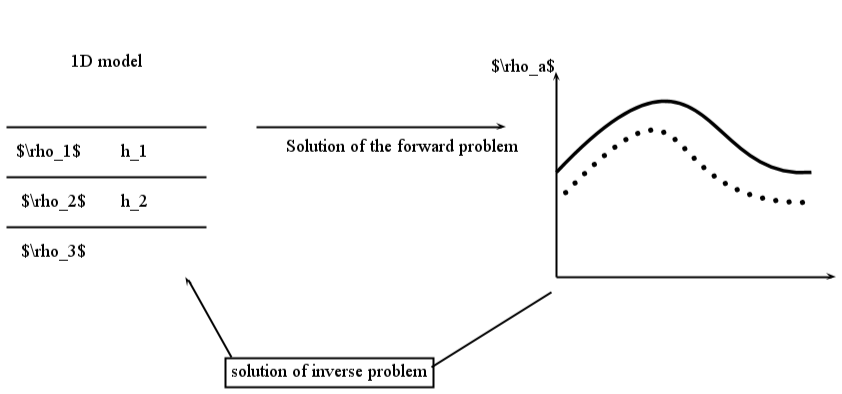
\includegraphics[width=0.7\textwidth]{invidea.eps}
\caption{Inversion idea}
\label{fig:inv01}
\end{center}
\end{figure}
The aim of the inversion is the minimization of the error function or cost function $\psi_d$ between observed and calculated apparent resistivity data. Minimize:
\begin{equation}
\psi_d=\|\vec{y}-f(\vec{m})\|^2
\end{equation}
$\vec{y}$ is the vector of measured data (e.g. $\vec{y}=(\rho_a(L/2=5m),\rho_a(L/2=10m),...)$.

$f(\vec{m}$ is the vector of calculated data.

$\psi_d$ is the norm of differences between measured and observed data.

\subsubsection{Strategies for the inversion}
Different methods to minimize the difference between measured and calculated data:
\begin{itemize}
\item Trial and error
\item method of Zohdy
\item Automatic inversion by linearisation of the forward operator $f(\vec{m})$
\end{itemize}

\paragraph{Trial and Error}

\begin{figure}[H]
\begin{center}
\resizebox{0.5\textwidth}{!}
{
\begin{pspicture}(0,-2.6034896)(7.9042706,2.6034896)
\usefont{T1}{ptm}{m}{n}
\rput(3.2217708,2.2642188){\psframebox[linewidth=0.04]{Input: Starting model $m_0$ and $y$=data}}
\usefont{T1}{ptm}{m}{n}
\rput(3.326302,0.76421875){\psframebox[linewidth=0.04]{Forward calculation $\rightarrow f(m_0)$}}
\usefont{T1}{ptm}{m}{n}
\rput(3.006302,-0.53578126){\psframebox[linewidth=0.04]{RMS small?}}
\usefont{T1}{ptm}{m}{n}
\rput(3.0766146,-2.2357812){\psframebox[linewidth=0.04]{Output: end model}}
\psline[linewidth=0.04cm,arrowsize=0.05291667cm 2.0,arrowlength=1.4,arrowinset=0.4]{->}(3.0367708,1.9592187)(3.0367708,1.0592188)
\psline[linewidth=0.04cm,arrowsize=0.05291667cm 2.0,arrowlength=1.4,arrowinset=0.4]{->}(3.0367708,0.45921874)(3.0367708,-0.24078125)
\psline[linewidth=0.04cm,arrowsize=0.05291667cm 2.0,arrowlength=1.4,arrowinset=0.4]{->}(3.0367708,-0.8407813)(3.0367708,-1.9407812)
\psline[linewidth=0.04cm](4.036771,-0.54078126)(7.1367707,-0.54078126)
\psline[linewidth=0.04cm](7.1367707,-0.54078126)(7.1367707,1.3592187)
\psline[linewidth=0.04cm,arrowsize=0.05291667cm 2.0,arrowlength=1.4,arrowinset=0.4]{->}(7.1367707,1.3592187)(3.1367707,1.3592187)
\usefont{T1}{ptm}{m}{n}
\rput(3.608802,-1.2357812){Yes}
\usefont{T1}{ptm}{m}{n}
\rput(7.6528645,0.26421875){No, new model}
\end{pspicture} 
}
\caption{Trial and error scheme}
\label{fig:trialanderror}
\end{center}
\end{figure}

with
\begin{equation}
RMS=\sqrt{\frac{1}{N}\sum_{i=1}^{N}\frac{(\rho_a^m(i)-\rho_a^c(i))^2}{(\rho_a^c(i))^2}}
\end{equation}
$\rho_a^m$ measured data, $\rho_a^c$ calculated data.

\paragraph{ZOHDY-technique}
This method is suitable for the inversion of DC-resistivity data measured by a four electrode array (Schlumberger, Wenner, ...).Utilize the principle of equivalence: The fitting of the measured data by using a resistivity model with a \textit{large} number of layers has the same quality if less layers are used.

\subsubsection*{Example:}
\begin{figure}[H]
\begin{center}
\resizebox{0.6\textwidth}{!}
{
\begin{pspicture}(0,-2.4329689)(14.081875,2.4329689)
\psline[linewidth=0.04cm,arrowsize=0.05291667cm 2.0,arrowlength=1.4,arrowinset=0.4]{->}(0.0,2.2345312)(0.0,-1.7654687)
\psline[linewidth=0.04cm,arrowsize=0.05291667cm 2.0,arrowlength=1.4,arrowinset=0.4]{->}(0.0,2.2345312)(4.0,2.2345312)
\psline[linewidth=0.04cm,arrowsize=0.05291667cm 2.0,arrowlength=1.4,arrowinset=0.4]{->}(8.0,-1.7654687)(8.0,2.2345312)
\psline[linewidth=0.04cm,arrowsize=0.05291667cm 2.0,arrowlength=1.4,arrowinset=0.4]{->}(8.0,-1.7654687)(13.1,-1.7654687)
\usefont{T1}{ptm}{m}{n}
\rput(13.611406,-2.2604687){$L/2$}
\usefont{T1}{ptm}{m}{n}
\rput(7.8214064,2.2395313){$\rho_a$}
\psline[linewidth=0.04cm](1.5,2.1345313)(1.5,1.1345313)
\psline[linewidth=0.04cm](1.5,1.1345313)(3.2,1.1345313)
\psline[linewidth=0.04cm](3.2,1.1345313)(3.2,-0.06546875)
\psline[linewidth=0.04cm](3.2,-0.06546875)(1.3,-0.06546875)
\psline[linewidth=0.04cm](1.3,-0.06546875)(1.3,-1.6654687)
\psline[linewidth=0.04cm](1.5,1.9345312)(1.7,1.9345312)
\psline[linewidth=0.04cm](1.7,1.9345312)(1.7,1.6345313)
\psline[linewidth=0.04cm](1.7,1.6345313)(1.6,1.6345313)
\psline[linewidth=0.04cm](1.6,1.6345313)(1.6,1.3345313)
\psline[linewidth=0.04cm](1.6,1.3345313)(1.9,1.3345313)
\psline[linewidth=0.04cm](1.9,1.3345313)(1.9,1.0345312)
\psline[linewidth=0.04cm](1.9,1.0345312)(2.2,1.0345312)
\psline[linewidth=0.04cm](2.2,1.0345312)(2.2,0.83453125)
\psline[linewidth=0.04cm](2.2,0.83453125)(2.5,0.83453125)
\psline[linewidth=0.04cm](2.5,0.83453125)(2.5,0.53453124)
\psline[linewidth=0.04cm](2.5,0.53453124)(2.8,0.53453124)
\psline[linewidth=0.04cm](2.8,0.53453124)(2.8,0.33453125)
\psline[linewidth=0.04cm](2.8,0.33453125)(3.3,0.33453125)
\psline[linewidth=0.04cm](3.3,0.33453125)(3.3,0.23453125)
\psline[linewidth=0.04cm](3.3,0.23453125)(2.9,0.23453125)
\psline[linewidth=0.04cm](2.9,0.23453125)(2.9,0.03453125)
\psline[linewidth=0.04cm](2.9,0.03453125)(2.5,0.03453125)
\psbezier[linewidth=0.106000006,linestyle=dotted,dotsep=0.16cm](8.0,-0.45008412)(8.0,-1.0654688)(9.5,1.9345312)(13.0,-0.06546875)
\psbezier[linewidth=0.106000006](8.1,-0.35008413)(8.1,-0.96546876)(9.1,2.0345314)(12.6,0.03453125)
\end{pspicture} 
}
\caption{Example layers in inversion}
\label{fig:inv02}
\end{center}
\end{figure}
\subsubsection*{Procedure}
\begin{compactenum}[1)]
\item Starting model with $m$ layers, where $m$ is the number of measured data. $\rho_i=\rho_{a_i}$, $t_i=(L/2)_i$. Thickness of the $i$'th layer: $h_i=(L/2)_{i+1}-(L/2)_{i}$.
Then do the forward and RMS calculation. For example RMS is 62\%.

\item Reduction of the thickness of each layer as 0.9 and then do forward and RMS calculation. Repetition of the procedure until no improvement of RMS is possible.
For example: 10 iterations reduce RMS to 12\%.

\item Determination of resistivity of each layer:
\begin{align*}
\rho_{i+1}(j)=\rho_i(j)\frac{\rho_{a_{i,obs}}(j)}{\rho_{a_{i,c}}(j)}
\end{align*}
with $i$ the number of iterations and $j$ the number of layer = $L/2$ number. $\rho_i(j)$: resistivity of the $j$'th layer of the $i$'th iteration. $\rho_{a_{i,c}}$: calculated apparent resistivity data for the $j$'th layer and $i$'th iteration.

Now do the forward calculation and calculate the RMS. Similar to step 2) repetition of the procedure (example 12\% to 1\%).
\end{compactenum}
\subsubsection*{Disadvantage:}
No good result, if data points have relatively large noise, because every data point is a layer.

\paragraph{Inversion by linearization of the forward operator}
The aim of the inversion is to minimize the cost function $\psi_d$. A measure for the error:
\begin{equation}
X^2=\frac{1}{N}\sum_{i=1}^{N}\frac{(y_i-f_i)^2}{\sigma_i^2}
\end{equation}
where $n$ is the number of measured data and calculated data. $\sigma$ is the standard deviation. 
\textit{Mathematically:} $\min \|y-f(m)\|^2$ (To solve use e.g. Gauss Newton method). The problem is not linear, therefore linearise $f(m)$ or $\psi_d$.

The linearisation can be done by a Taylor expansion of the forward operator $f(m)$ for small model changes $\Delta m$ close to the starting model $m_0$:
\begin{align}
f(m_0+\delta m)=f(m_0)+\frac{\partial f(m_0)}{\partial m_0}\Delta m\approx f(m_0)+\tens{J}\Delta m
\end{align}
where $\tens{J}$ is the jacobian or sensitivity matrix. It describes the influence of model parameters on the model response. eq. 2.38 can now be written as:
\begin{equation}
\psi_d(m_a)=\|y-f(m_0)\|^2=(y-f(m_0))^T(y-f(m_0))
\end{equation}
using the Taylor expansion:
\begin{equation}
\psi_d(m_0+\Delta m)=\|y-f(m_0+\Delta m)\|^2=(y-f(m_0+\Delta m))^T(y-f(m_0+\Delta m))
\end{equation}
Set eq. 2.40 in eq. 2.42
\begin{equation}
\psi_d(m_0+\Delta m)=\|y-f(m_0)-\tens{J}\Delta m\|^2=(y-f(m_0)-\tens{J}\Delta m)^T(y-f(m_0)-\tens{J}\Delta m)
\end{equation}
Calculation of the extreme of $\psi_d$:
\begin{align*}
\frac{\partial \psi_d(m_0+\Delta m)}{\partial \Delta m}=0=\frac{\partial }{\partial \Delta m}(y-f(m_0)-\tens{J}\Delta m)^T(y-f(m_0)-\tens{J}\Delta m)
\end{align*}
with $\Delta d=y-f(m_0)$:
\begin{align*}
0&=\frac{\partial }{\partial \Delta m}(\Delta d-\tens{J}\Delta m)^T(\Delta d-\tens{J}\Delta m)\\
&=\frac{\partial }{\partial \Delta m}(\Delta d^T\Delta d-\Delta d^T\tens{J}\Delta m-\Delta m J^T\Delta d +\Delta m^TJ^TJ\Delta m)\\
&=2J^T\Delta d-2J^TJ\Delta m\\
\Leftrightarrow J^TJ\Delta m&=J^T\Delta d
\end{align*}
Normal equation: Solution for this equation according to $\Delta m$
\begin{equation}
\Delta m=(J^TJ)^{-1}J^T\Delta d\label{eq:solutioninv}
\end{equation}
For the linear case the minima of $\psi_d$ can be reached after one iteration. For the non-linear case $m_1=m_0+\Delta m$, $m_2=m_1+\Delta m$, so the solution will be iteratively improved!


\textit{Problem:} No solution of \eqref{eq:solutioninv} if $(J^T J)$ is singular, or in other words $\det(J^TJ)=0$. To stabilize it
\begin{align*}
\Delta m(J^TJ+\beta I)^{-1}J^T\Delta d
\end{align*}
with $\beta$ the damping factor and $I$ the identity matrix. The solution according to the eq. is known as \textit{Marquardt-Levenberg method}.

\subsection{Solution of the 2D DC forward problem}
\begin{figure}[H]
\begin{center}
\resizebox{0.6\textwidth}{!}
{
\begin{pspicture}(0,-1.5789063)(12.715625,1.5589062)
\psline[linewidth=0.04cm](0.0,0.5389063)(9.0,0.5389063)
\psline[linewidth=0.04cm](3.0,0.5389063)(3.0,-0.86109376)
\psline[linewidth=0.04cm](3.0,-0.86109376)(5.0,-0.86109376)
\psline[linewidth=0.04cm](5.0,-0.86109376)(5.0,0.5389063)
\psline[linewidth=0.04cm,linestyle=dashed,dash=0.16cm 0.16cm](3.0,0.5389063)(5.0,1.5389062)
\psline[linewidth=0.04cm,linestyle=dashed,dash=0.16cm 0.16cm](5.0,0.5389063)(7.0,1.5389062)
\usefont{T1}{ptm}{m}{n}
\rput(3.9014063,-0.15609375){$\sigma_2$}
\usefont{T1}{ptm}{m}{n}
\rput(1.9014063,-1.3560938){$\sigma_1$}
\psline[linewidth=0.04cm,arrowsize=0.05291667cm 2.0,arrowlength=1.4,arrowinset=0.4]{->}(11.0,0.5389063)(11.0,-0.86109376)
\psline[linewidth=0.04cm,arrowsize=0.05291667cm 2.0,arrowlength=1.4,arrowinset=0.4]{->}(11.0,0.5389063)(12.4,0.5389063)
\psline[linewidth=0.04cm,arrowsize=0.05291667cm 2.0,arrowlength=1.4,arrowinset=0.4]{->}(11.0,0.5389063)(12.0,1.2389063)
\usefont{T1}{ptm}{m}{n}
\rput(12.585468,0.44390625){x}
\usefont{T1}{ptm}{m}{n}
\rput(12.287812,1.3439063){y}
\usefont{T1}{ptm}{m}{n}
\rput(11.2734375,-0.9560937){z}
\end{pspicture} 
}

\caption{asdfasdf}
\label{fig:solution2DDC}
\end{center}
\end{figure}

\subsubsection*{Basic equations:}
Ohm's law:
\begin{align*}
j=\sigma E\\
E=-\nabla V\\
j=-\sigma \nabla V
\end{align*}
By using the charge retention over a volume, the continuity equation can now be written as:
\begin{equation}
\nabla j=\frac{\partial q}{\partial t}\delta(x)\delta(y)\delta(z)\label{eq:poisson02}
\end{equation}
The charge density $q$ is represented at a point in the cartesian coordinates $(x,y,z)$ with the Dirac-distribution $\delta(x)$.

\begin{align}
-\nabla\left(\sigma(x,y,z)\nabla V(x,y,z)\right)=\frac{\partial q}{\partial t}\delta(x_s)\delta(y_s)\delta(z_s)
\end{align}
The \textit{Poisson equation}, with $x_s,y_s,z_s$ the coordinates of the source point. By using the vector equation $\nabla\cdot (\phi A) = \nabla\phi A +\phi\nabla \cdot A)$ with $A=\nabla V$ and $\phi=\sigma$. Then the equation \eqref{eq:poisson02} will be:
\begin{equation}
\nabla\sigma(x,y,z)\nabla V(x,y,z)+\sigma(x,y,z)\nabla^2 V(x,y,z)=-\frac{\partial q}{\partial t}\delta(x_s)\delta(y_s)\delta(z_s)\label{eq:poisson03}
\end{equation}
No change of electrical conductivity in y-direction so we have a 2D problem. $\Rightarrow \frac{\partial}{\partial y}\sigma(x,y,z)=0$.

Application of this condition to \eqref{eq:poisson02} and \eqref{eq:poisson03}:
\begin{align}
-\nabla\cdot(\sigma\nabla V)&=\frac{\partial q}{\partial t}\delta(x_s)\delta(y_s)\delta(z_s)\\
\nabla\sigma\cdot\nabla V+\sigma\nabla^2 V&=-\frac{\partial q}{\partial t}\delta(x_s)\delta(y_s)\delta(z_s)
\end{align}
Using the vector equation: $\nabla A\cdot\nabla B=\frac{1}{2}(-A\nabla^2 B + \nabla^2(AB)-B\nabla^2 A)$ with $A=\sigma$ and $B=V$ we get:

\begin{align*}
\nabla^2(\sigma(x,z)V(x,y,z))+\sigma(x,z)\nabla^2 V(x,y,z)-V(x,y,z)\nabla^2\sigma(x,z)=-2\frac{\partial q}{\partial t}\delta(x_s)\delta(y_s)\delta(z_s)
\end{align*}
Spatial distribution of the potential $V \rightarrow$ 3D, spatial distribution of the conductivity $\sigma \rightarrow$ 2D. Therefore the solution in this form is not possible.

The $y$-dependence of the potential can now be eliminated by the \textit{Fourier-cosine transformation}:
\begin{align*}
\tilde{V}(x,K_y,z)=\int\limits_{0}^{\infty}V(x,y,z)\cos(K_y y)dy
\end{align*}
3D $V(x,y,z)$ is due to point source at $(x_s,y_s,z_s)$ over a 2D conductivity structure is reduced to a 2D transformed potential $\tilde{V}(x,K_y,z)$, with $K_y$ the wave number.

For $\tilde{V}(x,K_y,z)$ the solution

\begin{align}
\nabla^2(\sigma(x,z)\tilde{V}(x,K_y,z))+\sigma(x,z)\nabla^2 \tilde{V}(x,K_y,z)-\tilde{V}(x,K_y,z)\nabla^2\sigma(x,z)-2K_y\sigma(x,z)\tilde{V}(x,K_y,z)=-2Q\delta(x_s)\delta(z_s)\label{eq:vtildeeq}
\end{align}
is looked for with $Q\delta(x_s)\delta(z_s)=\frac{1}{2}\frac{\partial q}{\partial t}$

The relationship between the stationary current density $Q$ and the current:

\begin{align*}
Q=\frac{I}{2\Delta A}
\end{align*}
where $\Delta A$ is the area around the current electrodes.

The eq. \eqref{eq:vtildeeq} is solved for different wave numbers. Afterwards do the inverse transformation:

\begin{equation*}
V(x,y,z)=\frac{2}{\pi}\int\limits_{0}^{\infty}\tilde{V}(x,K_y,z)\cos(K_y y)dK_y
\end{equation*}
Numerical solution of \eqref{eq:vtildeeq} with \textit{boundary conditions} (2D forward modelling). The boundary conditions are:

\begin{compactenum}[a)]
\item $V(x,y,z)$ is continuous between two media with different conductivity $\sigma$.
\item $V(x,y,z)\rightarrow 0$ if $z\rightarrow\infty$
\item $j_n$ is also continuous
\end{compactenum}

Now discretization of the subsurface and solution of \eqref{eq:vtildeeq} with (for example) finite differences:

\begin{figure}[H]
\begin{center}
\resizebox{0.4\textwidth}{!}
{
\begin{pspicture}(0,-2.7417188)(5.414375,2.7617188)
\psline[linewidth=0.04cm](0.394375,2.2782812)(0.394375,-2.7217188)
\psline[linewidth=0.04cm](1.394375,2.2782812)(1.394375,-2.7217188)
\psline[linewidth=0.04cm](2.394375,2.2782812)(2.394375,-2.7217188)
\psline[linewidth=0.04cm](3.394375,2.2782812)(3.394375,-2.7217188)
\psline[linewidth=0.04cm](4.394375,2.2782812)(4.394375,-2.7217188)
\psline[linewidth=0.04cm](0.394375,2.2782812)(5.394375,2.2782812)
\psline[linewidth=0.04cm](0.394375,1.2782812)(5.394375,1.2782812)
\psline[linewidth=0.04cm](0.394375,0.27828124)(5.394375,0.27828124)
\psline[linewidth=0.04cm](0.394375,-0.7217187)(5.394375,-0.7217187)
\psline[linewidth=0.04cm](0.394375,-1.7217188)(5.394375,-1.7217188)
\usefont{T1}{ptm}{m}{n}
\rput(0.24125,2.4832811){1}
\usefont{T1}{ptm}{m}{n}
\rput(1.3729688,2.5832813){2}
\usefont{T1}{ptm}{m}{n}
\rput(2.3620312,2.5832813){3}
\usefont{T1}{ptm}{m}{n}
\rput(3.3753126,2.5832813){4}
\usefont{T1}{ptm}{m}{n}
\rput(0.07296875,1.2832812){2}
\usefont{T1}{ptm}{m}{n}
\rput(0.06203125,0.28328124){3}
\usefont{T1}{ptm}{m}{n}
\rput(0.0753125,-0.71671873){4}
\psline[linewidth=0.04cm,arrowsize=0.05291667cm 2.0,arrowlength=1.4,arrowinset=0.4]{->}(6.494375,-0.42171875)(3.994375,-0.32171875)
\usefont{T1}{ptm}{m}{n}
\rput(7.795781,-0.41671875){$\sigma = const$}
\end{pspicture} 
}
\caption{Finite differences grid}
\label{fig:fdgrid}
\end{center}
\end{figure}
Calculation of the potential at the knots of the mesh and afterwards $\rho_a=K\frac{\Delta V}{I}$

